%! Author = sbbfti
%! Date = 10/06/2020


\section{Results}\label{sec:results}

The sensible heat losses from the skin to the environment are proportional to the difference between the \ac{t-sk} and \ac{t-op}, as shown in Equation~\ref{eq:c-r}.
Consequently for values of \ac{t-op} higher than \ac{t-sk} the term \ac{c-r} becomes negative and the body gains sensible heat from its environment.
Figure~\ref{fig:comparison_models}A shows how the sensible heat losses estimated with the \mycite{GaggeSET} and the \mycite{Jay2015} models vary as a function of the \ac{t-op}, \ac{rh}, and \ac{v}.
The former model iteratively determines \ac{t-sk}, while the latter assumes it to be constant and equal to 35~°C.
This explains the difference in \ac{c-r} determined by the two models.
For \ac{t-op} higher than those at which \ac{w-max} occurs (Figure~\ref{fig:comparison_models}B), our model estimates that heat energy gets stored in the body and consequently \ac{t-sk} increases, as shown in Figure~\ref{fig:results_model_2}C.
This reduces the sensible heat gains estimated by our model when compared with the results obtained by \mycite{Jay2015}.
The values of \ac{w} and the respective values of \ac{w-max} for two air speeds are shown in Figure~\ref{fig:comparison_models}B.

\begin{figure}[b!]
    \centering
    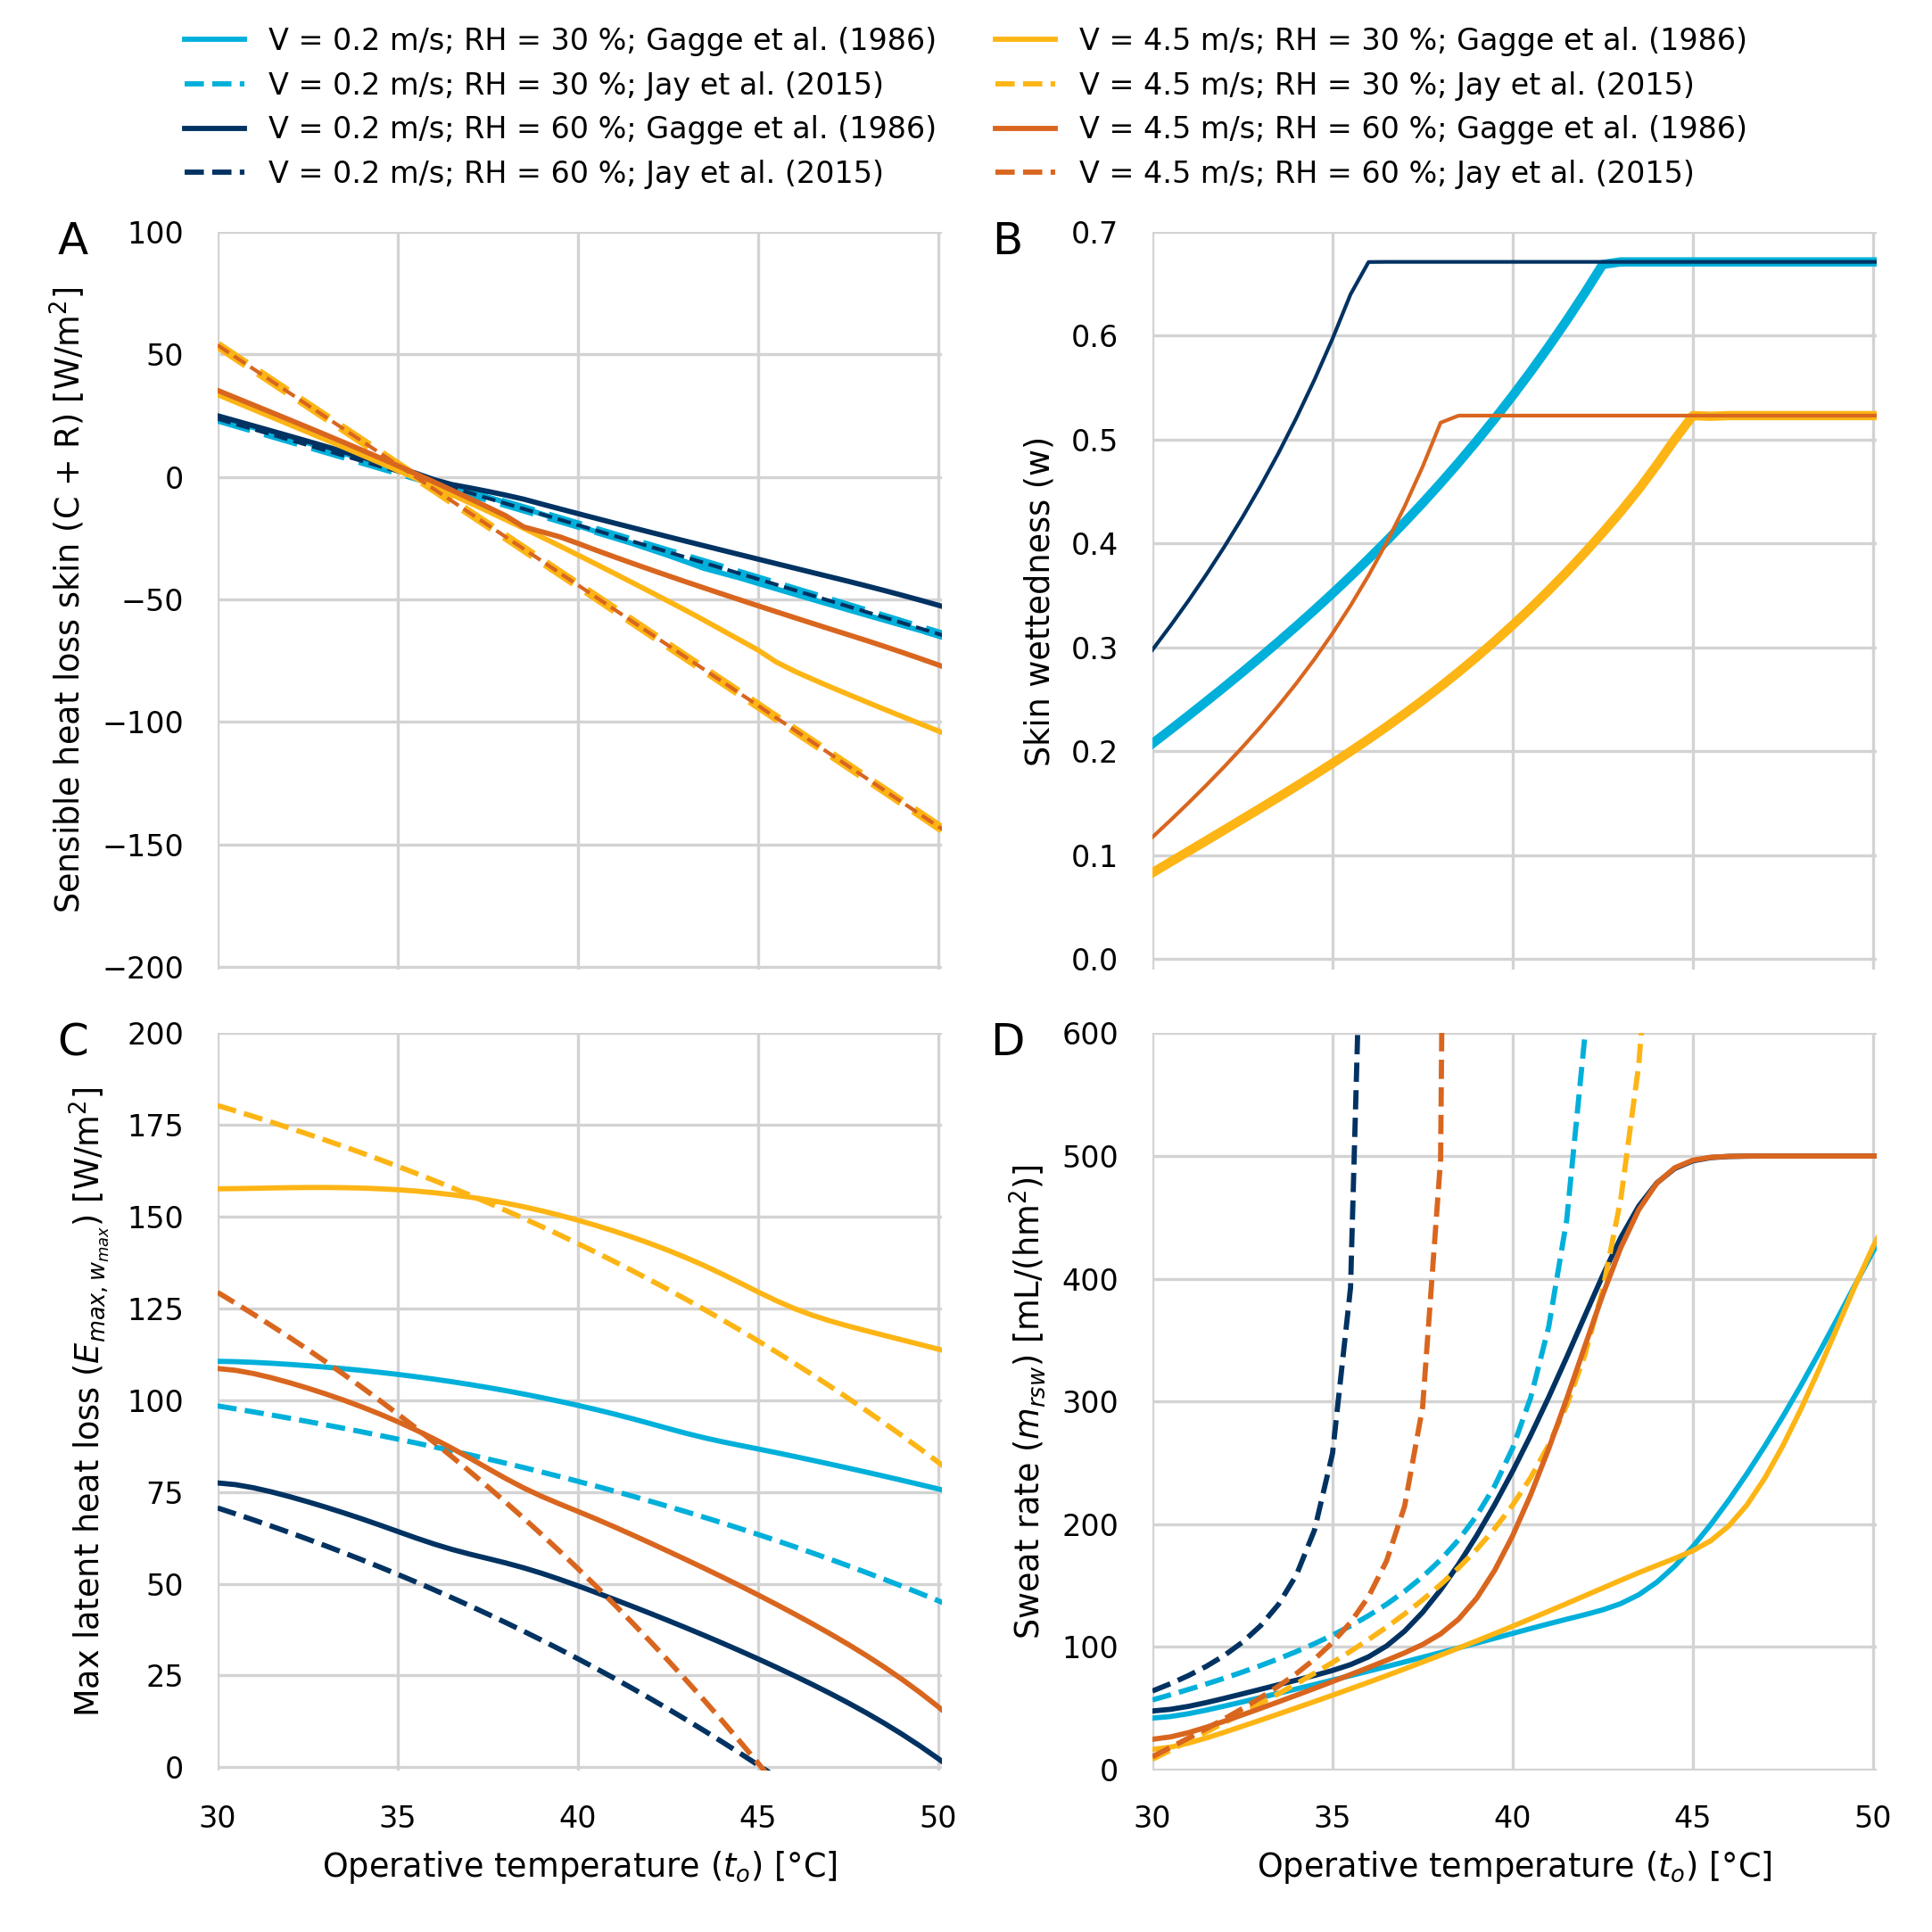
\includegraphics[width=\textwidth]{figures/comparison_models_v2.png}
    \caption{Shows how the results obtained with the the energy models proposed by \mycite{Jay2015} and \mycite{GaggeSET} vary as a function of the \ac{t-op}.
    Each Figure shows the results obtained using a combination of two values of \ac{rh} and \ac{v}.
    Figure A - sensible heat losses from the skin vary.
    Figure B - skin wettendess.
    Figure C - Maximum latent heat loss estimated using \ac{w} = \ac{w-max}.
    Figure D - Sweat rate.}
    \label{fig:comparison_models}
\end{figure}

The negative effect that an increase in \ac{v} has on the sensible heat gains is, however, compensated by a larger increase in the value of \ac{e-sk} that the body can dissipate towards the environment.
For example, when \ac{t-op}~=~45~°C and \ac{rh}~=~30~\%, an increase in \ac{v} from 0.2 to 4.5~m/s increases the sensible heat gains (\acs{c-r}) by 29 W/m\textsuperscript{2} while \ac{e-sk} increases by 45~W/m\textsuperscript{2}, hence, it has a net positive effect.
Figure~\ref{fig:comparison_models}C shows the values of \ac{e-max} estimated by replacing \ac{w} in Equation~\ref{eq:latent-skin} with \ac{w-max}.
The value of \ac{e-max} decreases as the \ac{t-op} increases since \ac{p-a} grows more rapidly than \ac{p-sk}.
The reduction in \ac{e-max} estimated by our model is lower than the one estimated by \mycite{Jay2015} since the former assumes that the skin temperature increases as the value of \ac{t-op} increases.
For a set combination of \ac{v} and \ac{t-op} the value of \ac{e-max} decreases as the value of \ac{rh} increases since humid air has a higher \ac{p-a} than dry air.
Finally, it can be observed that for a fixed increase in \ac{v}, the relative increase in \ac{e-max} decreases as the \ac{rh} increase.

Figure~\ref{fig:comparison_models}D shows the estimated \ac{m-sweat}.
The difference between the results obtained with the two heat balance models can be attributed to the fact that \citeauthor{Jay2015} calculates the value of \ac{m-sweat} as a function of only the required latent energy that the body should in theory dissipate to achieve thermal neutrality.
However, \citeauthor{GaggeSET} assumes that the human body cannot always achieve thermal neutrality in all conditions (as shown in Figure~\ref{fig:results_model_2}B) and consequently for a set of specific environmental conditions the value of \ac{e-sk} has an upper limit.
This in turns affect the value of \ac{m-sweat}.
Moreover, conversely to \citeauthor{Jay2015}, \citeauthor{GaggeSET} assumes that \ac{m-sweat} cannot exceed 500~mL/h.

\begin{figure}[b!]
    \centering
    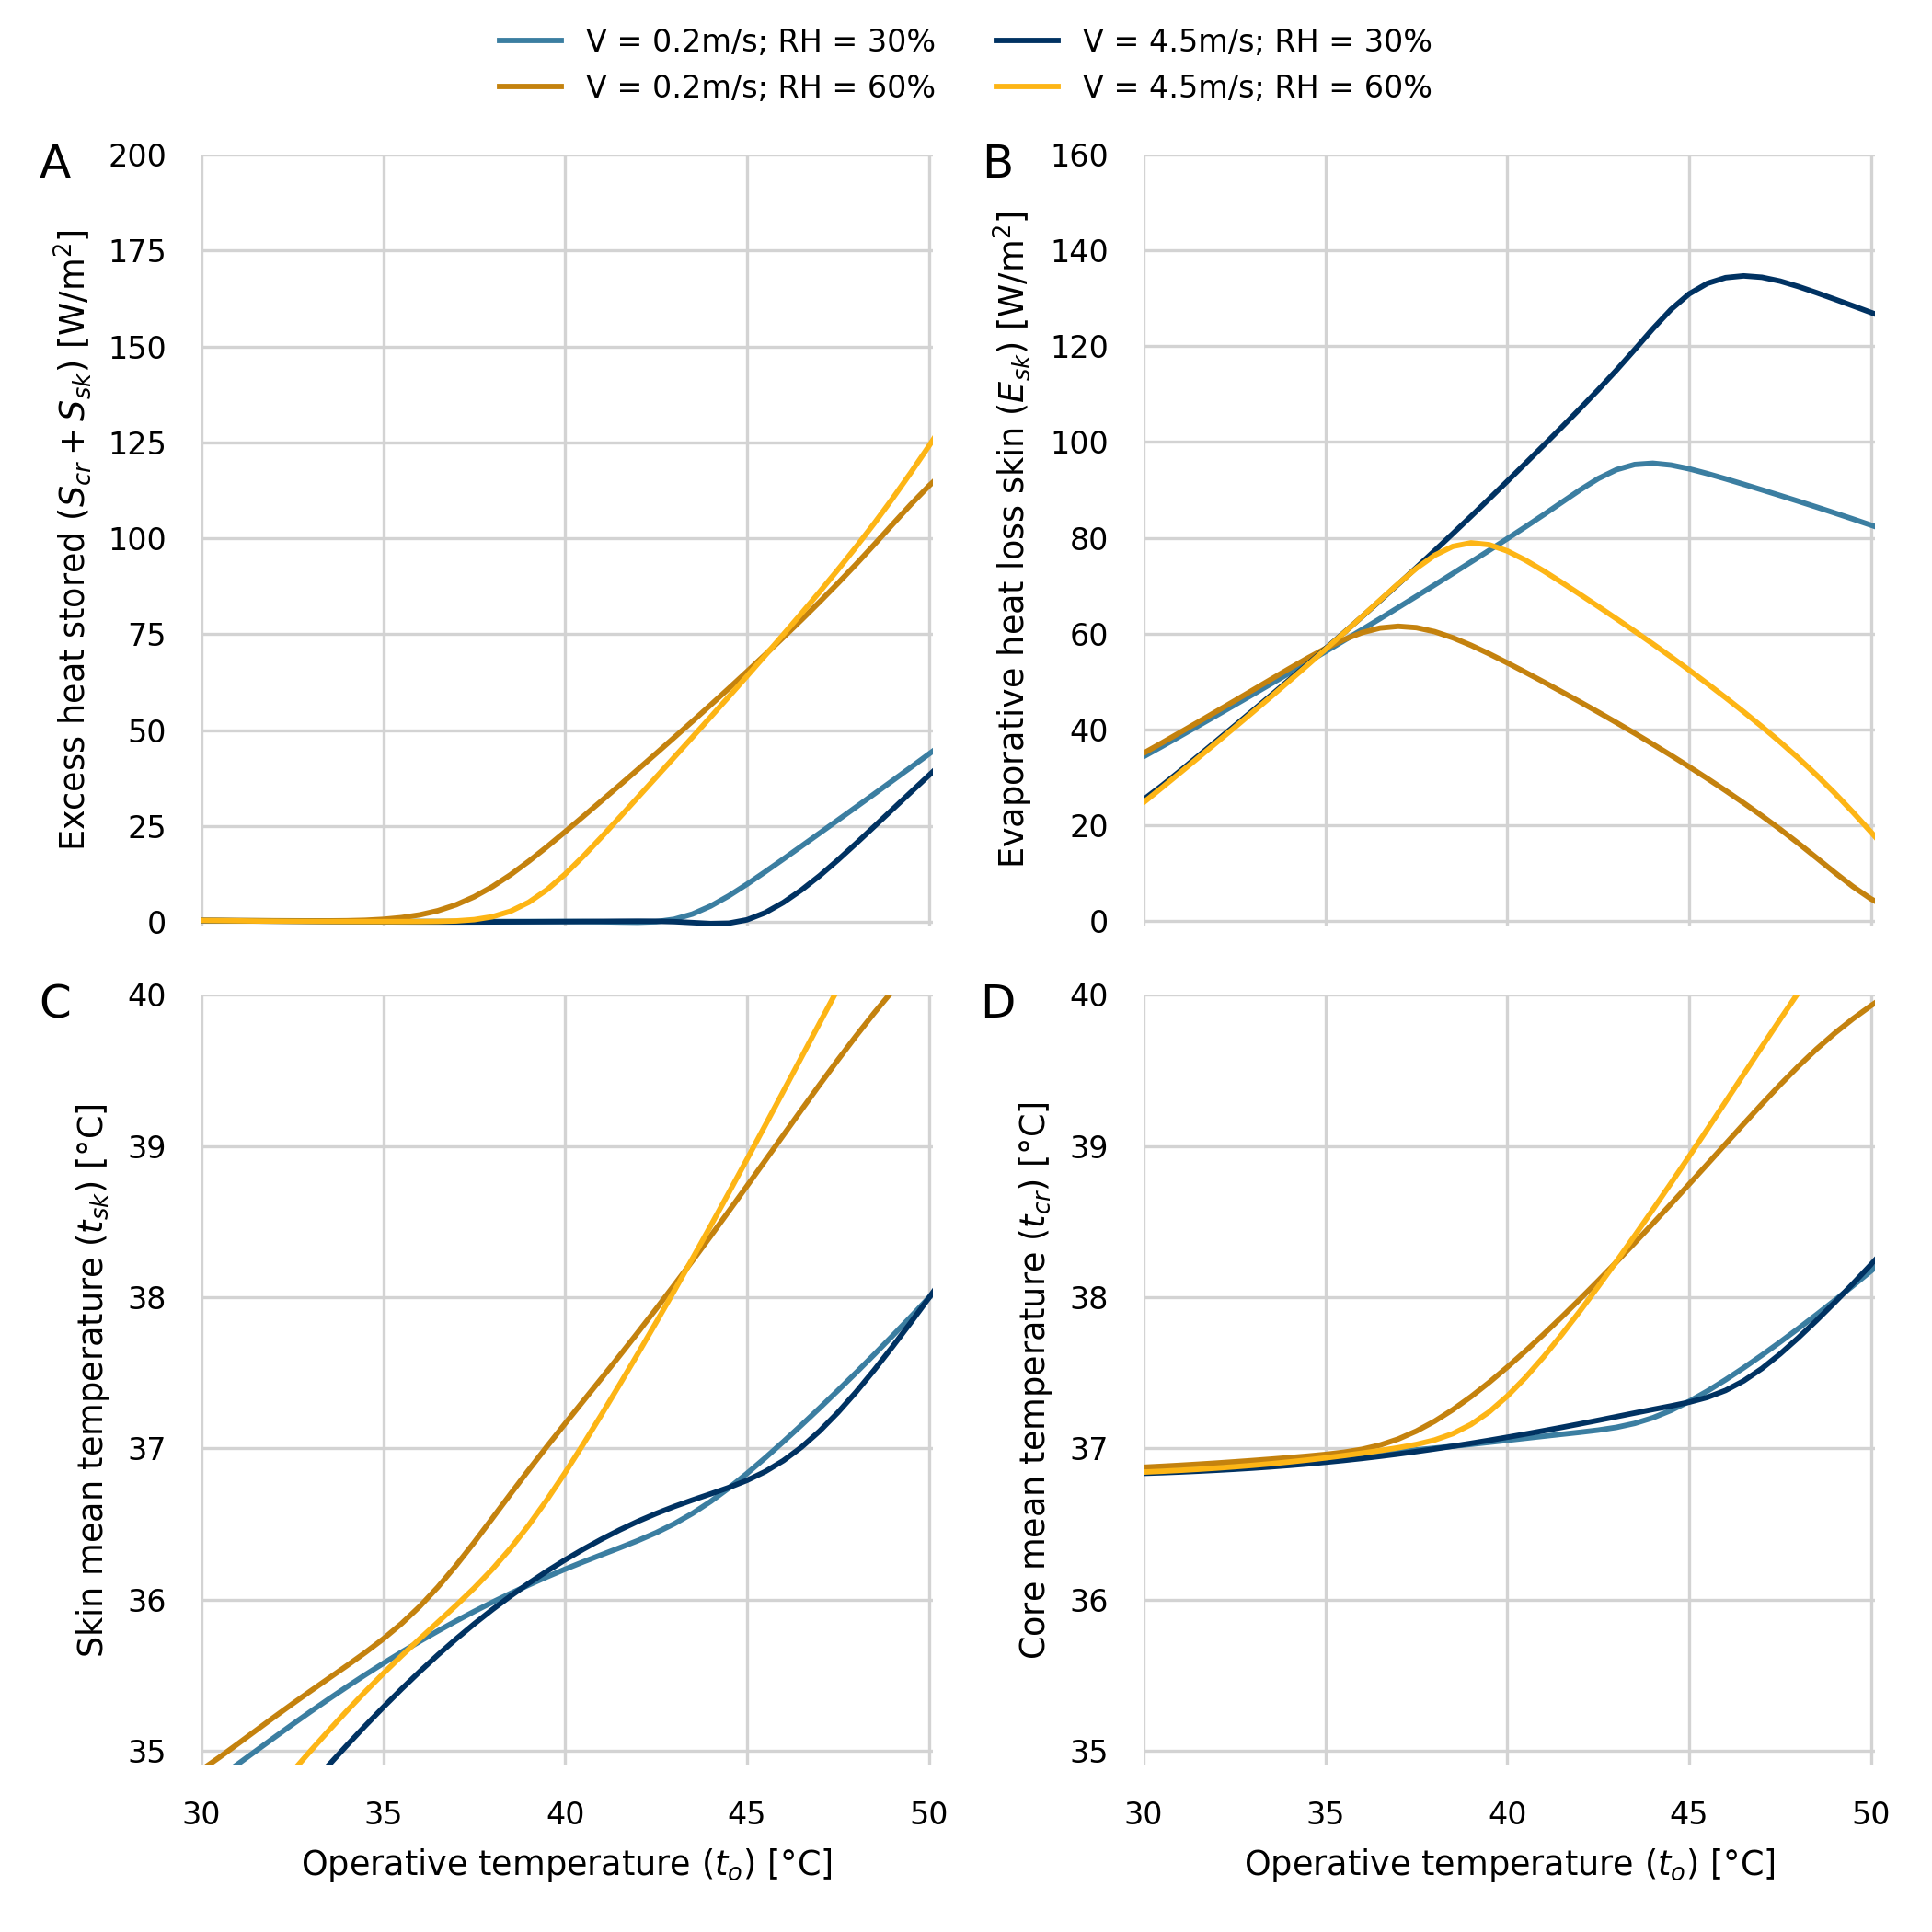
\includegraphics[width=\textwidth]{figures/results_model_2.png}
    \caption{Caption}
    \label{fig:results_model_2}
\end{figure}

The estimated values of \ac{t-cr} and excess heat stored in the human body are shown in Figure~\ref{fig:results_model_2}D and ~\ref{fig:results_model_2}A, respectively.
The two values are related to each other and as soon as the body cannot longer dissipate the exogenous and endogenous heat gains, the excess heat gets stored in the body and causes an increase in both \ac{t-sk} and \ac{t-cr}.
The \ac{t-op} at which the energy stored in the human body with elevated air speed exceeds the `still air' condition is when the use of air movement becomes detrimental.
While, when the energy stored becomes greater than 0 is the conditions which demarcates when heat strain would start to occur.

The combination of \ac{t-op}, \ac{rh}, and \ac{v} at which heat strain would start to occur since the body is no longer able to dissipate all the heat gains are presented in Figure~\ref{fig:comparison_air_speed}.
The Figure shows both the results obtained with the\mycite{GaggeSET} and the \mycite{Jay2015} models.
It should be noted that the limit presented in Figure~\ref{fig:comparison_air_speed} is not the limit above which an increase in \ac{v} is no longer beneficial.
Each line demarcates the region in which thermal stress is estimated to occur and not all individuals would be able to compensate for endogenous and exogenous heat gains.
For a specific value of \ac{v}, the maximum \ac{t-op} at which cardiovascular strain is estimated to occur decreases as the value of \ac{rh} increases.
In addition, it can be observed that for a specific value of \ac{rh}, as the value of \ac{v} increases the overall increase in the maximum critical temperature rapidly decreases.
For example, in an environment with \ac{rh}~=~60~\%, increasing \ac{v} from 0.1~m/s to 0.8~m/s then to 4.5~m/s lead to an increase of the critical temperature of approximately 2.3~°C and 0.8~°C, respectively.

The environmental conditions above which the use of elevated air speeds would actually be detrimental for the health of the people is shown in Figure~\ref{fig:energy_storage_delta}.
This figure depicts the environmental conditions above which the heat balance model would estimate that the \ac{t-cr} would be higher with \ac{v} of XX~m/s rather than with 0.1~m/s.
This would occur since the sensible heat gains caused by forced convection, would exceed the heat losses from the body towards its surrounding environment.

% todo report estimated sweat heat lossess too, either using a table or a heatmap


%\begin{itemize}
%    \item I do not really see the benefit of the model proposed by Hosper since: 1) they set the limit of sweating to 440 mL/h; and they limit 2) the amount of water than I person can spray on him self to 116 mL/h. This would not affect the results in the SET model since with the SET model the estimated sweating rate is lower.
%    On the other hand it affects the result in the Ollie model since the exponential growth of the sweat rate in their model is more marked.
%    Moreover, very dry climates could benefit from using evaporative cooling.
%\end{itemize}

\begin{figure}
    \centering
    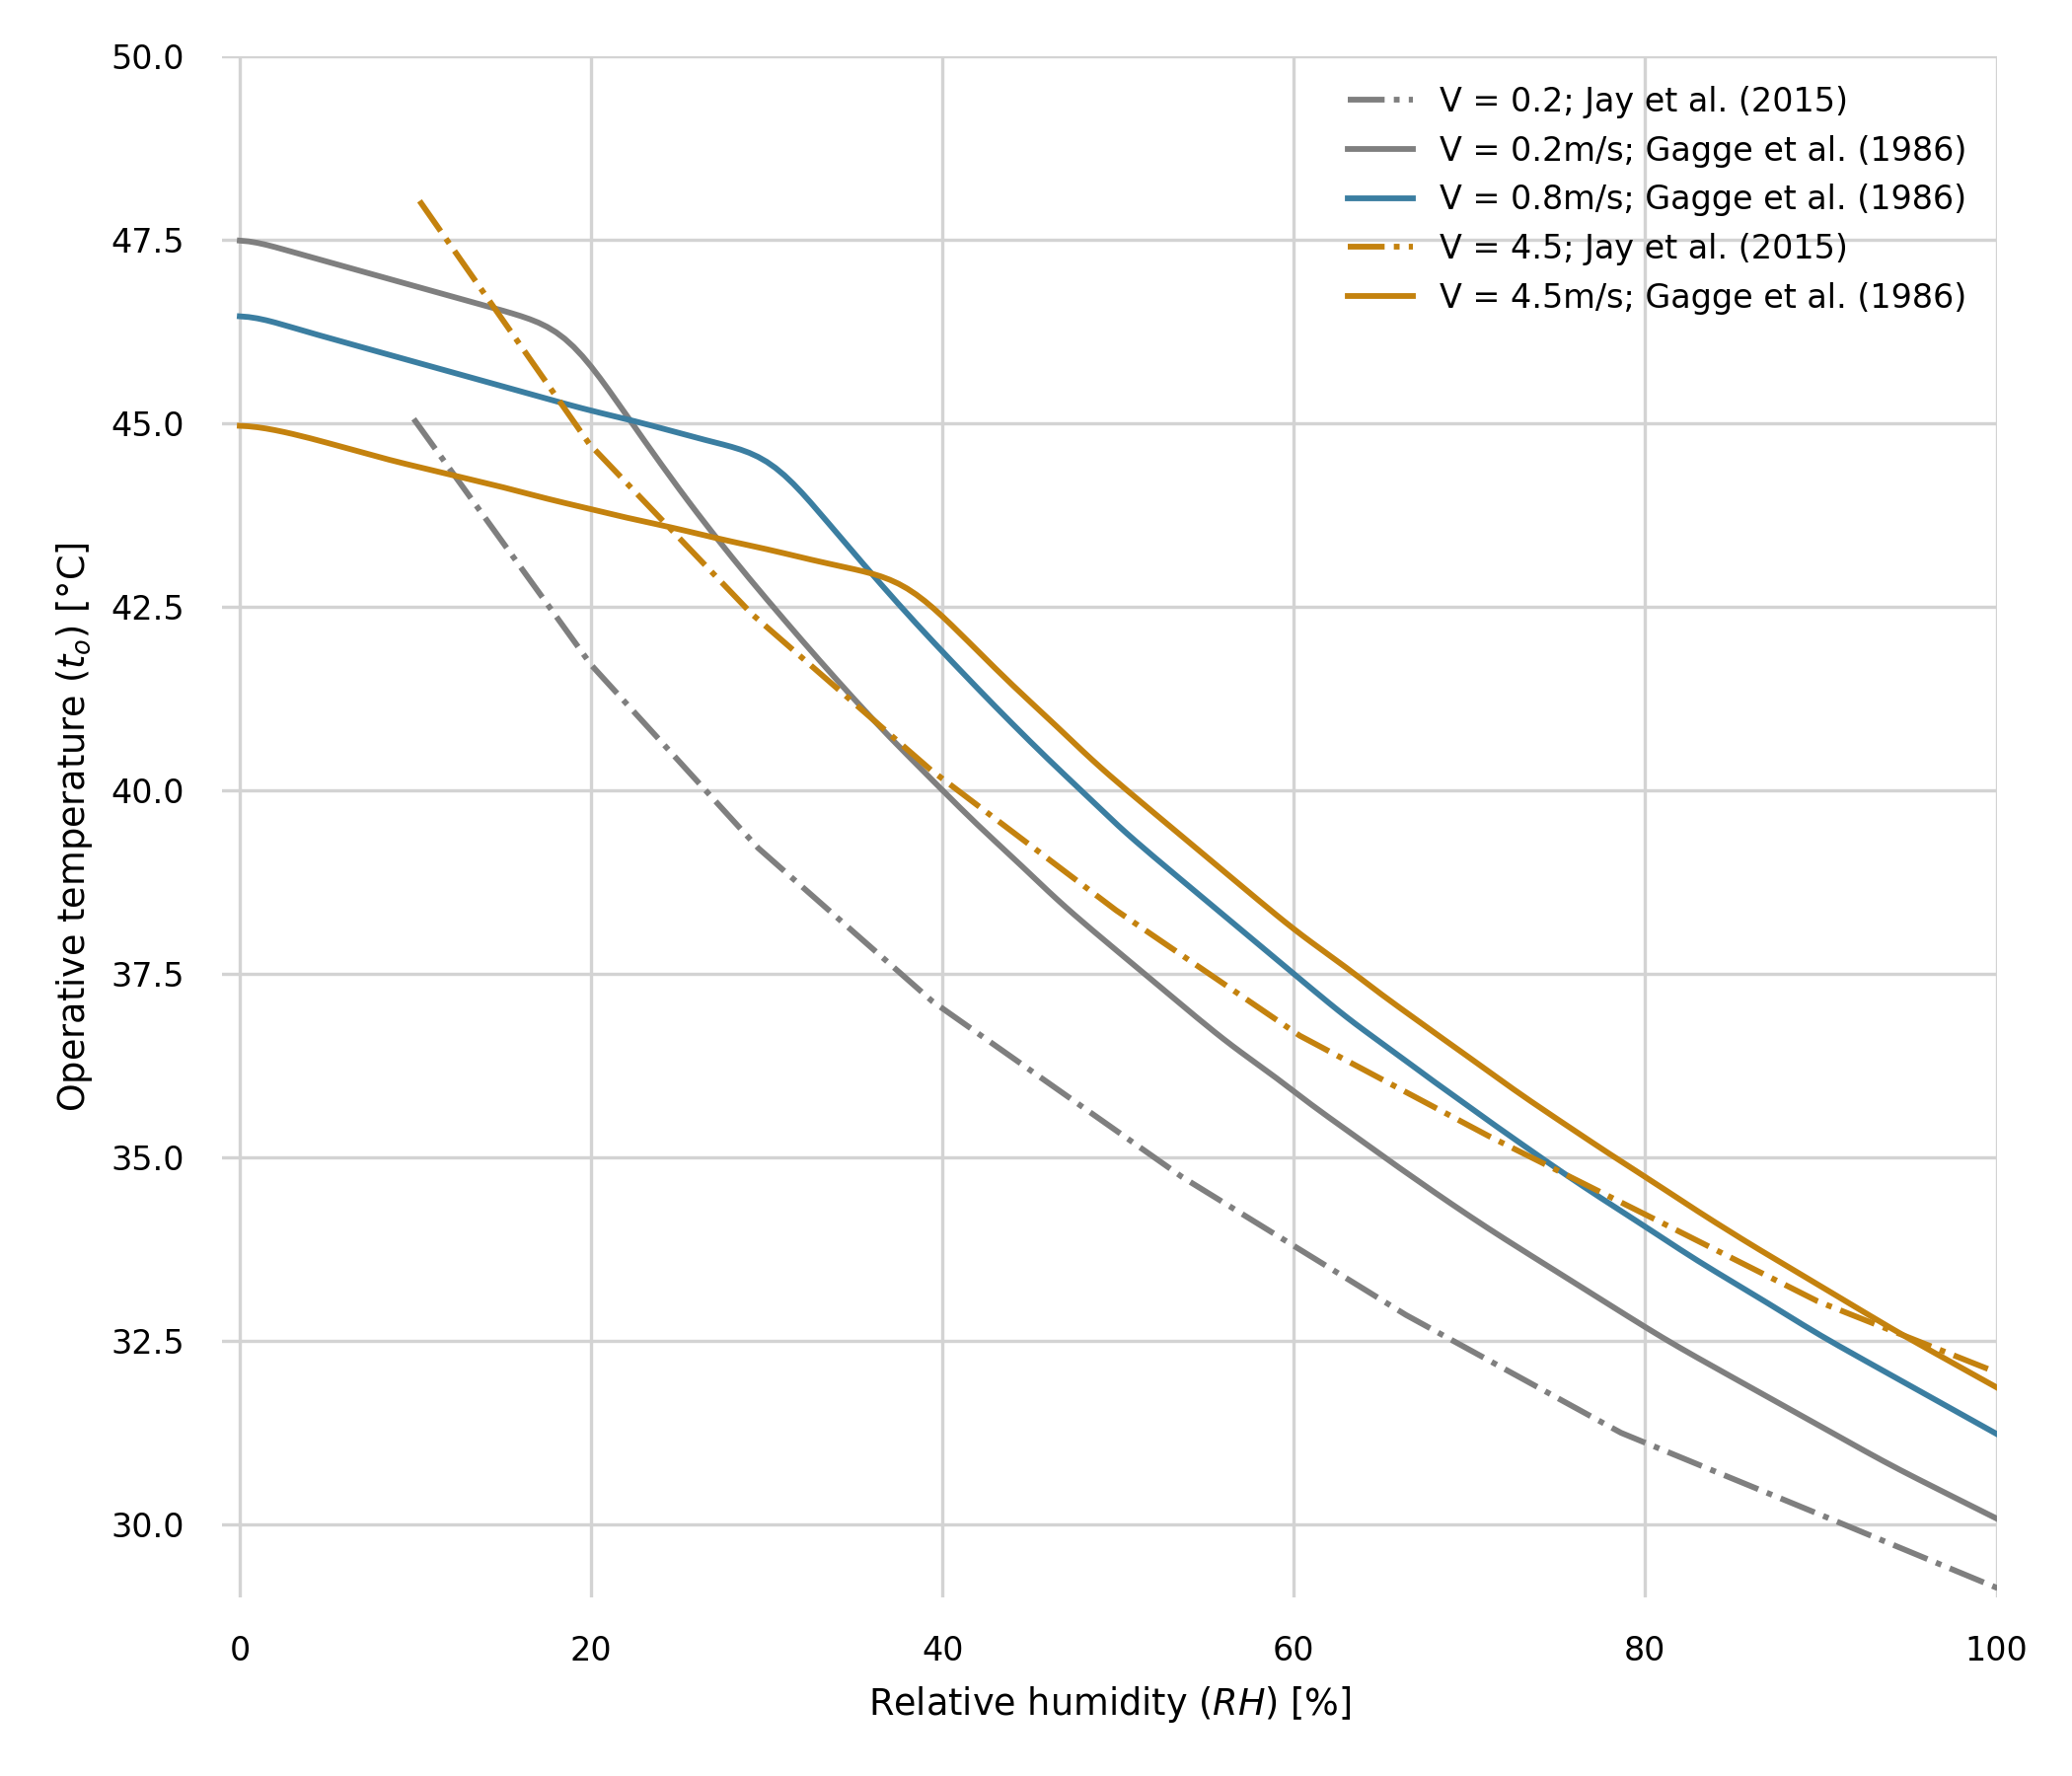
\includegraphics[width=\textwidth]{figures/comparison_air_speed.png}
    \caption{Compares the results between the SET model and Ollie's model.
    Each line demarcates the boundary between acceptable cardiovascular strain (below line) and elevated cardiovascular strain (above the line).
    Above the line the latent heat that needs to be dissipated exceeds the amount of latent heat that the same individual can dissipate. }
    \label{fig:comparison_air_speed}
    % todo extend the lines to the top left border, add units to axis and change label to opertative temperature
\end{figure}

\begin{figure}
    \centering
    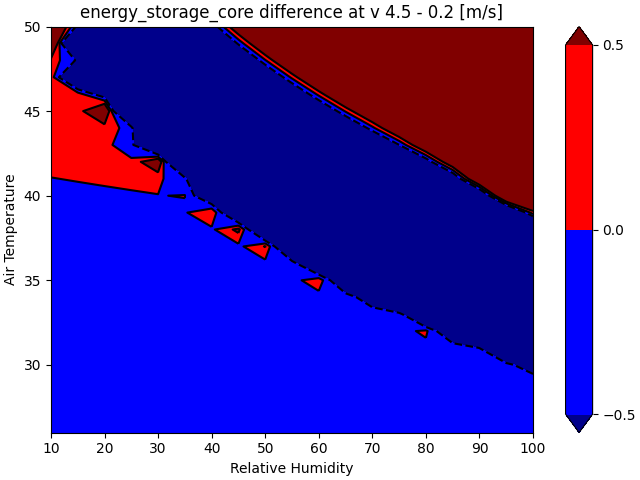
\includegraphics[width=\textwidth]{figures/energy_storage_delta.png}
    \caption{Caption}
    \label{fig:energy_storage_delta}
%    todo replace this figure with the core body delta
\end{figure}


